\section{Личный вклад в развитие проекта}

В рамках данной курсовой работы я занимался разработкой двух ключевых микросервисов: \textbf{messenger} (для общения пользователей) и \textbf{reactions} (для обработки реакций пользователей на предложения для общения других пользователей).

\textbf{Messenger:} 
Для реализации сервиса messenger я использовал Java 21 и Spring Boot 3 с подключением к базе данных ScyllaDB. Я спроектировал таблицу для хранения сообщений с учетом всех ограничений ScyllaDB. Структура таблицы выглядит следующим образом:

\begin{figure}[h]
    \begin{verbatim}
    create table if not exists messages
    (
        companions_composite_key text,
        id                       timeuuid,
        sender_id                uuid,
        recipient_id             uuid,
        date                     timestamp,
        content                  text,
        tag_name                 text,
        tag_external_id          uuid,
        PRIMARY KEY (companions_composite_key, id)
    ) with clustering order by (id desc);
    \end{verbatim}
    \caption{Описание таблицы с сообщениями в базе данных}
\end{figure}

В данной таблице:
\begin{itemize}
    \item \textbf{companions\_composite\_key} используется как разделяющий ключ для обеспечения равномерного распределения данных по узлам кластера.
    \item \textbf{id} (timeuuid) используется как кластеризующий ключ для упорядочивания сообщений по дате отправки в порядке убывания.
    \item \textbf{sender\_id} и \textbf{recipient\_id} идентифицируют отправителя и получателя сообщения.
    \item \textbf{date} хранит временную метку отправки сообщения.
    \item \textbf{content} содержит текст сообщения.
    \item \textbf{tag\_name} и \textbf{tag\_external\_id} используются для добавления меток к сообщениям.
\end{itemize}

Для данного сервиса API был спроектирован с использованием OpenAPI, что обеспечило стандартизацию и удобство интеграции с другими компонентами системы. Пример документации API представлен на рисунке \ref{swagger_messenger} и \ref{swagger_reactions}.

\begin{figure}[h]
    \centering
    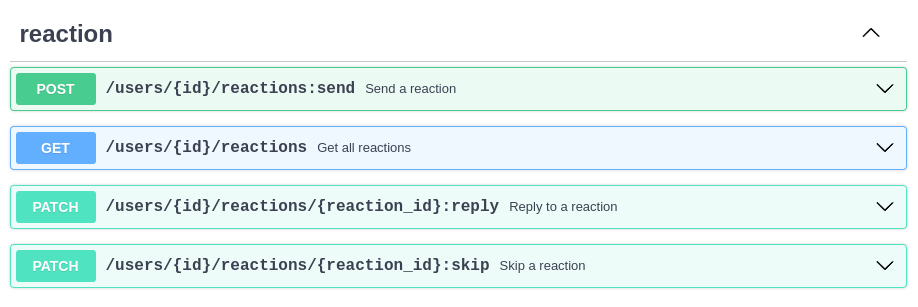
\includegraphics[width=1\linewidth]{swagger_reactions.png}
    \caption{Скриншот из Swagger UI с документацией API сервиса reactions}
    \label{swagger_reactions}
\end{figure}

\begin{figure}[h]
    \centering
    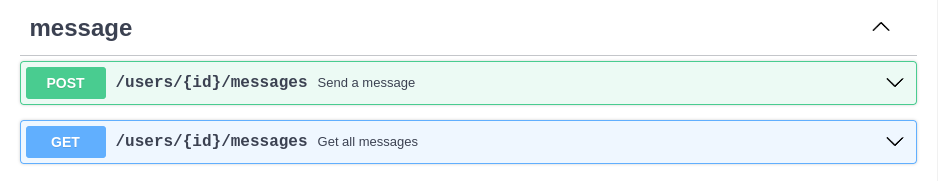
\includegraphics[width=1\linewidth]{swagger_messenger.png}
    \caption{Скриншот из Swagger UI с документацией API сервиса messenger}
    \label{swagger_messenger}
\end{figure}

\textbf{Reactions:} 
Сервис reactions был разработан на базе Spring Boot 3 и Java 21 с подключением к базе данных PostgreSQL. Данный микросервис интегрируется с сервисами profiles и messenger через gRPC, что обеспечивает эффективное взаимодействие и передачу данных между компонентами системы.

\textbf{Процесс развертывания:}
Я также разработал и реализовал процесс развертывания приложения, начиная от создания pull request до загрузки контейнеров в реестр Docker. Пример выполнения процесса можно увидеть на рис. \ref{ci_pipeline}. 

\begin{figure}[h]
    \centering
    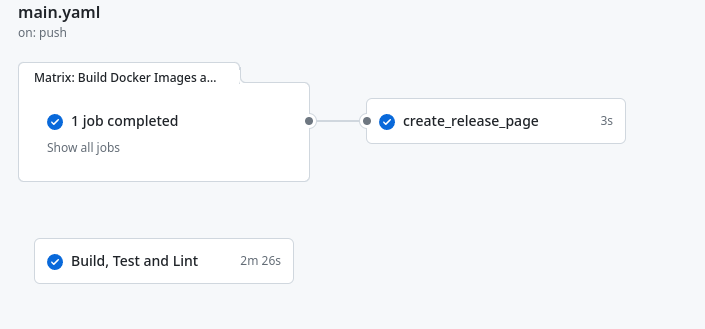
\includegraphics[width=1\linewidth]{ci_pipeline.png}
    \caption{Скриншот из Github Actions с процессом CI/CD}
    \label{ci_pipeline}
\end{figure}

\textbf{Развертывание окружений:}
В рамках этой работы были развернуты два окружения: тестовое и продуктовое.

\begin{itemize}
    \item \textbf{Тестовое окружение:} Развернуто на виртуальной машине в cloud.ru (бывший sbercloud) с использованием Minikube. Это позволило нам проводить интеграционные и нагрузочные тестирования в условиях, максимально приближенных к боевым.
    \item \textbf{Продуктовое окружение:} Развернуто на полноценном кластере Managed Kubernetes от cloud.ru с 16 vCPU и 32 ГБ RAM с использованием Helm charts. В данном окружении были развернуты все компоненты бэкенда, Kubernetes Dashboard и Loki-stack для мониторинга. Пример состояния кластера можно увидеть на рис. \ref{kubernetes_dashboard}.
\end{itemize}

\textbf{Мониторинг и дашборды:}
Для мониторинга состояния системы и визуализации метрик я развернул Grafana и настроил дашборды, которые предоставляют графики и показатели производительности. Это включает метрики состояния микросервисов, использования ресурсов и задержек запросов, что позволяет оперативно отслеживать и устранять возможные проблемы в работе системы. Пример дашборда для сервиса messenger представлен на рис. \ref{grafana_dasboard}.

\begin{figure}[h!]
    \centering
    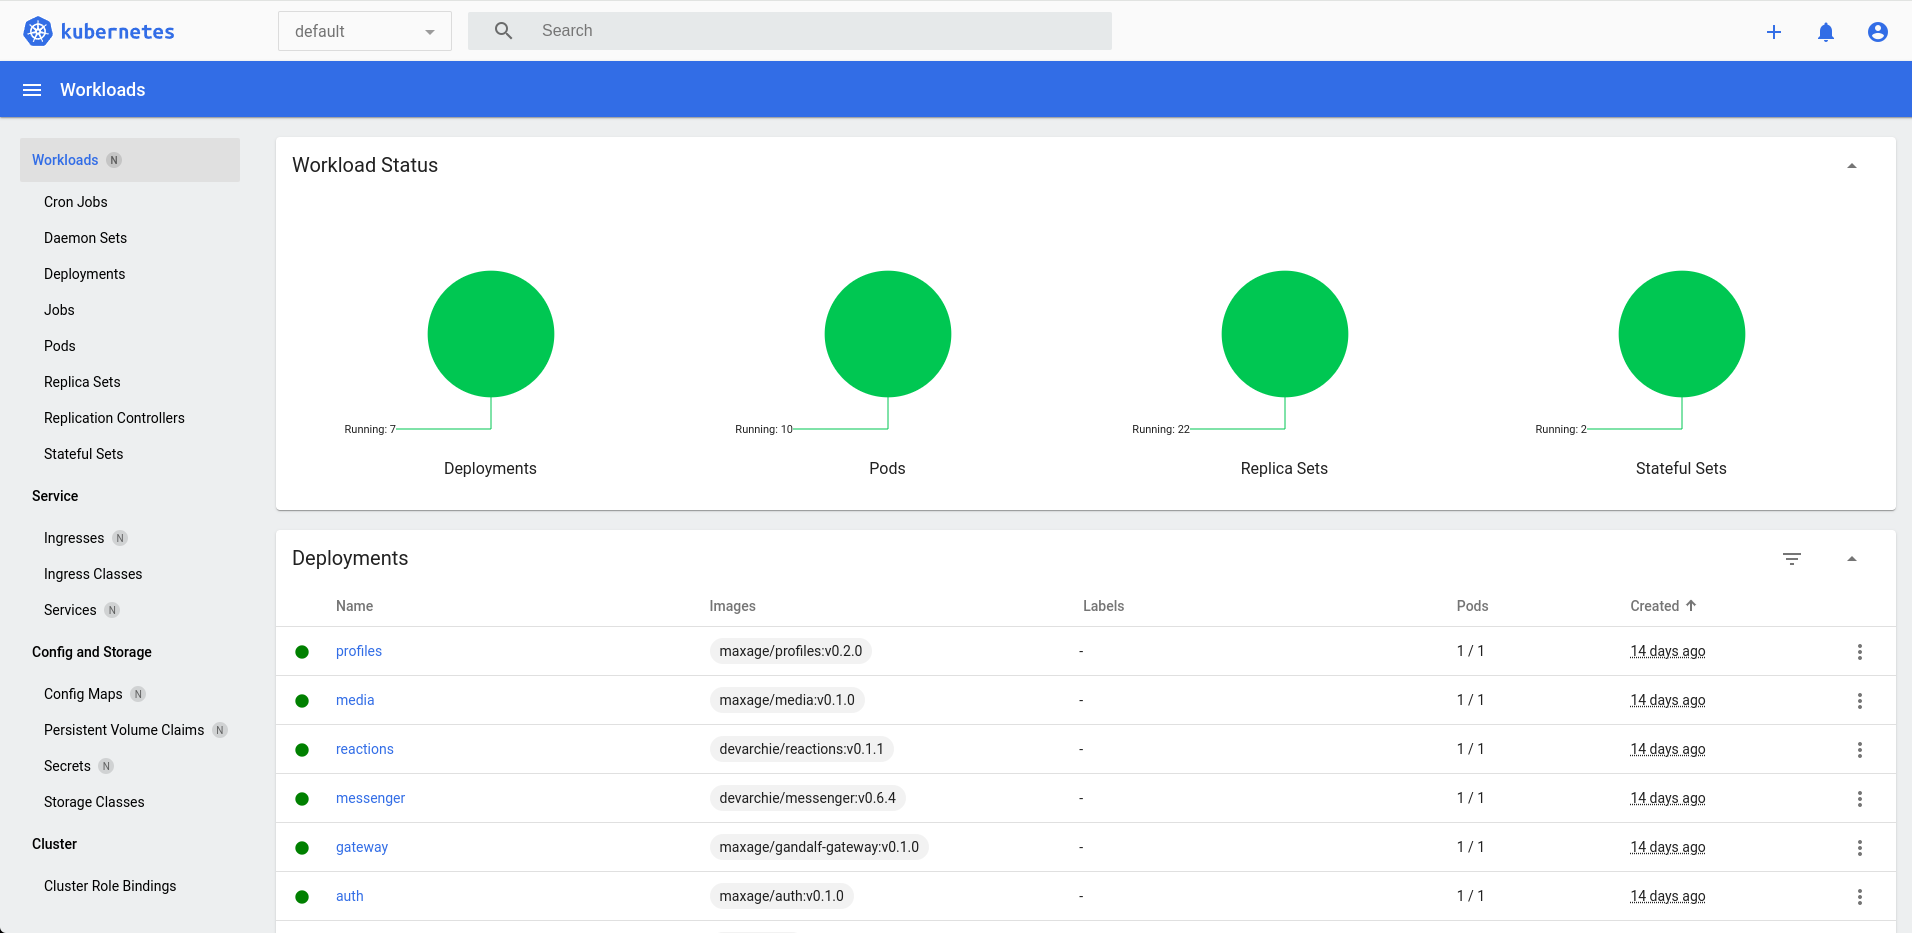
\includegraphics[width=1\linewidth]{kubernetes_dasboard.png}
    \caption{Скриншот Kubernetes Dashboard с состоянием кластера}
    \label{kubernetes_dashboard}
\end{figure}

\begin{figure}[h!]
    \centering
    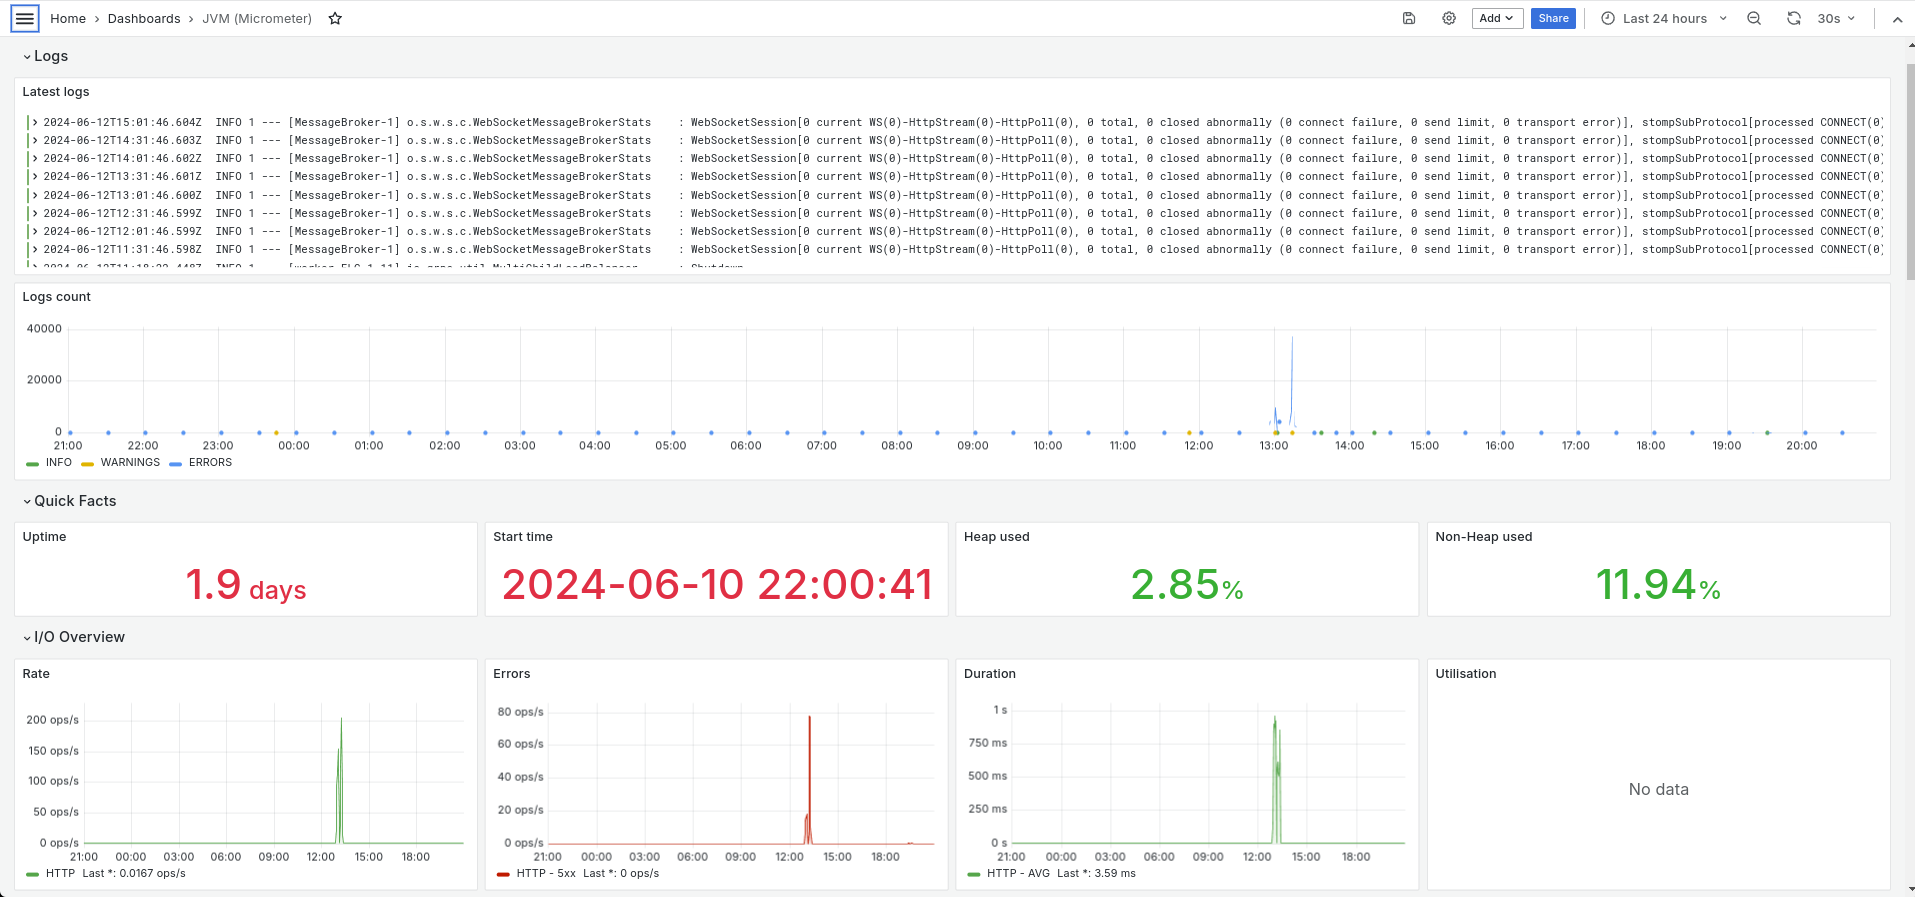
\includegraphics[width=1\linewidth]{grafana_dashboard.png}
    \caption{Скриншот с дашбордом Grafana для мониторинга метрик на примере сервиса messenger}
    \label{grafana_dasboard}
\end{figure}

Таким образом, мой личный вклад в проект включал разработку и реализацию ключевых микросервисов, настройку процессов CI/CD, развертывание и мониторинг тестовых и продуктовых окружений, что в совокупности обеспечило стабильную и производительную работу приложения.